% or aspectratio=43
\documentclass[aspectratio=169,handout]{beamer}

% remove this line for an english presentation
%\usepackage{ngerman}

% Optional arguments (separate by comma):
% darkmode			- Black background and white font
% imagetitlepage	- Adds the images defined in \titlegraphic to the title page
\usepackage[imagetitlepage]{lgdv/lgdv_beamer}

\usepackage{mdframed}

\usepackage{xcolor}
\graphicspath{{images/}}


\newcommand\ytl[2]{
	\parbox[b]{8em}{\hfill{\color{cyan}\bfseries\sffamily #1}~$\cdots\cdots$~}\makebox[0pt][c]{$\bullet$}\vrule\quad \parbox[c]{10.5cm}{\vspace{7pt}\color{red!80!black!80}\raggedright\sffamily #2\\[7pt]}\\[-3pt]}


\subtitle{AGPhys WS 18/19}
\title{Debugging and Profiling CUDA Kernels}
\author[Darius Rückert]{Darius Rückert}
\date{\today}

\titlegraphic
{
	\begin{figure}[!h]
					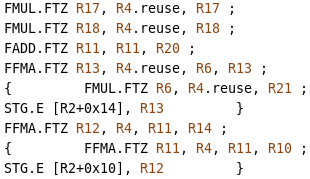
\includegraphics[height=.3\textheight]{sass2}
	\end{figure}
}

\begin{document}

\frame
{
	\titlepage
}


\frame
{
	\frametitle{CUDA Compilation}
		\begin{figure}
	\centering
	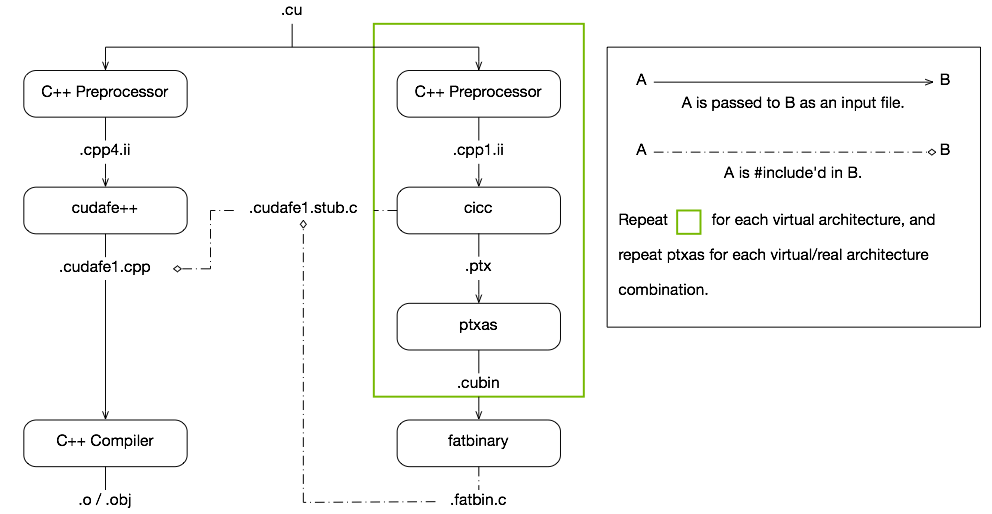
\includegraphics[height=0.95\textheight]{nvcc}
\end{figure}
}


\begin{frame}[fragile]
	\frametitle{Nvidia C Compiler (nvcc)}
	\begin{itemize}
		\item Supports C and C++
		\item Splits source files into host and device code
		\item Compiles device code to PTX and SASS
		\item Embeds the compiled device code in a synthetic C++ file
		\item Passes the generated C++ file to the host compiler (for example gcc)
	\end{itemize}	
Compiling a single source file into an executable named \textit{main}:
\begin{lstlisting}[language=bash]
nvcc -arch=sm_61 -g main.cu -o main
\end{lstlisting}
\end{frame}



\begin{frame}[fragile]
\frametitle{nvcc compiler flags}

\begin{itemize}
	
	\item[] \textbf{-g}
	\begin{itemize}
		\item[] Generate debug information for host code.
	\end{itemize}
	
		\item[] \textbf{-G}
	\begin{itemize}
		\item[] Generate debug information for device code. Turns off all optimizations. 
	\end{itemize}

	\item[] \textbf{-lineinfo}
\begin{itemize}
	\item[] Generate line-number information for device code.
\end{itemize}

\item[] \textbf{-src-in-ptx}
\begin{itemize}
	\item[] Interleave source in PTX. May only be used in conjunction with -G or -lineinfo. 
\end{itemize}

	\item[] \textbf{-ptx}
\begin{itemize}
	\item[] Compile all .cu input files to device-only .ptx files. This step discards the host code for each .cu input file. 
\end{itemize}

	\item[] \textbf{-V}
\begin{itemize}
	\item[]  	Print version information on this tool.
\end{itemize}

\end{itemize}
\end{frame}


\begin{frame}[fragile]
\frametitle{nvcc compiler flags}

\begin{itemize}
	\item[] \textbf{-arch}
	\begin{itemize}
		\item[] Specify the name of the class of NVIDIA virtual GPU architecture for which the CUDA input files must be compiled. 
	\end{itemize}
	
	\item[] \textbf{-code}
	\begin{itemize}
		\item[] Specify the name of the NVIDIA GPU to assemble and optimize PTX for. 
	\end{itemize}
	
	\item[] \textbf{-maxrregcount}
	\begin{itemize}
		\item[] Specify the maximum amount of registers that GPU functions can use. 
	\end{itemize}

	\item[] \textbf{-use\_fast\_math}
\begin{itemize}
	\item[] Make use of fast math library.
\end{itemize}


\item[] \textbf{-res-usage}
\begin{itemize}
	\item[] Show resource usage such as registers and memory of the GPU code. 
\end{itemize}

\end{itemize}
\end{frame}


\begin{frame}[fragile]
\frametitle{nvcc compiler flags}

\begin{itemize}
\item[] \textbf{-Xcompiler=[flag]}
\begin{itemize}
\item[] Passes [flag] to the CUDA host compiler
\end{itemize}

\item[] \textbf{--expt-relaxed-constexpr}
\begin{itemize}
\item[] Allows constexpr functions without \texttt{device} keyword to be used in device code
\end{itemize}

\item[] \textbf{--relocatable-device-code=true}
\begin{itemize}
\item[] Required for dynamic parallelism
\end{itemize}

\item[] \textbf{-restric}
\begin{itemize}
\item[] Assert that all kernel pointer parameters are restrict pointers.
\end{itemize}

\item[] \textbf{--profile}
\begin{itemize}
\item[] Instrument generated code/executable for use by gprof.
\end{itemize}


\end{itemize}
\end{frame}


\begin{frame}[fragile]
\frametitle{CUDA Compile Architectures}
	
		\begin{tabular}{c|l|l|l}
		Architecture & virtual arch flag & code flag & Graphic Cards\\	
		\hline
		Kepler & compute\_30 & sm\_30 & Geforce 700 Series\\
		Maxwell & compute\_52 & sm\_52 & Geforce 900 Series\\
		Pascal & compute\_61 & sm\_61 & Geforce 1000 Series\\
		Volta & compute\_70 & sm\_70 & Titan-V\\
		Turing & compute\_80 & sm\_80 & RTX 2000 Series\\	
	    Ampere & compute\_80 & sm\_80 & RTX 3000 Series\\	
	\end{tabular}
\\
	\vspace{0.6cm}
	Example command to compile for GTX 900 and 1000 Series:
\begin{lstlisting}[language=bash]
nvcc -gencode=arch=compute_52,code=sm_52 -gencode=arch=compute_61,code=sm_61 main.cu -o main
\end{lstlisting}
\end{frame}


\begin{frame}[fragile]
\frametitle{Just in time compilation (JIT)}
The PTX code for a virtual architecture can be embedded in a binary CUDA file. This will execute \texttt{ptxas} \textbf{at startup time} to compile the code for the current hardware. This has the following advantages/disadvantages:
\begin{itemize}
	\item Compiling is faster
	\item Starting the application takes longer
	\item Better compatibility to  different hardware
\end{itemize}
JIT can be enabled by repeating the virtual arch flag in the \texttt{code} flag:
\begin{lstlisting}[language=bash]
nvcc -gencode=arch=compute_30,code=compute_30 -gencode=arch=compute_61,code=sm_61 main.cu -o main
\end{lstlisting}
This example uses JIT for all architectures except sm\_61, because we told the compiler to generate SASS code for sm\_61.
\end{frame}

\begin{frame}[fragile]
\frametitle{NVCC and CMake}
\begin{itemize}
	\item The CUDA architecture is set by a target property
\end{itemize}
\begin{lstlisting}[language=bash]
set_property(TARGET hello_world PROPERTY 
	CUDA_ARCHITECTURES 52-virtual 61 70 80 )
\end{lstlisting}
\begin{itemize}
	\item Additional flags are appended to \texttt{CMAKE\_CUDA\_FLAGS} 
\end{itemize}
\begin{lstlisting}[language=bash]
list(APPEND MY_CUDA_FLAGS "-use_fast_math")
list(APPEND MY_CUDA_FLAGS "--expt-relaxed-constexpr")
list(APPEND MY_CUDA_FLAGS "-Xcompiler=-fopenmp")
list(APPEND MY_CUDA_FLAGS "-G")

# Add flags only to .cu files of the given target
target_compile_options(hello_world PRIVATE
  $<$<COMPILE_LANGUAGE:CUDA>:${MY_CUDA_FLAGS}>)
\end{lstlisting}

\end{frame}



\begin{frame}[fragile]
\frametitle{Parallel Thread Execution (PTX) ISA}
\begin{itemize}
	\item PTX is a low-level parallel thread execution virtual machine and instruction set architecture (ISA)
	\item Provides a stable ISA that spans multiple GPU generations.
	\item CUDA Device code is compiled to ptx and then from ptx to assembly
	\item \href{https://docs.nvidia.com/cuda/parallel-thread-execution/index.html}{PTX Documentation}
\end{itemize}
\textbf{Example \texttt{a[i] = b[i] + c[i]}:}
\begin{lstlisting}[language=bash]
add.s64 %rd8, %rd6, %rd7;
ld.global.f32 %f1, [%rd8];
add.s64 %rd9, %rd5, %rd7;
ld.global.f32 %f2, [%rd9];
add.f32 %f3, %f1, %f2;
add.s64 %rd10, %rd4, %rd7;
st.global.f32 [%rd10], %f3;
\end{lstlisting}
\end{frame}


\begin{frame}[fragile]
\frametitle{Shader Assembly (SASS)}
\begin{itemize}
\item SASS is the code executed by a specific GPU
\item Mostly similar to PTX, but
\begin{itemize}
	\item SASS is harder to read
	\item the documentation on SASS is a lot worse
\end{itemize}
\item \href{https://docs.nvidia.com/cuda/cuda-binary-utilities/index.html#maxwell-pascal}{Pascal Instruction Set reference}
\end{itemize}
\textbf{Example \texttt{a[i] = b[i] + c[i]}:}
\begin{lstlisting}[language=bash]
ISCADD R4.CC, R0, c[0x0][0x150], 0x2;
LD.E R2, [R2];              
IMAD.HI.X R5, R0, R7, c[0x0][0x154]; 
LD.E R4, [R4];            
ISCADD R6.CC, R0, c[0x0][0x140], 0x2; 
IMAD.HI.X R7, R0, R7, c[0x0][0x144];  
FADD R0, R2, R4; 
ST.E [R6], R0;    
\end{lstlisting}
\end{frame}


\begin{frame}[fragile]
	\frametitle{cuobjdump}
	\textbf{cuobjdump} extracts information from CUDA binary files. The extracted information include:
	\begin{itemize}
		\item CUDA assembly code for each kernel (SASS)
		\item Embedded PTX text
		\item CUDA ELF section headers
		\item String tables
		\item Relocators
	\end{itemize}	

\begin{lstlisting}[language=bash]
# Examples:
cuobjdump hello_world -ptx > ptx.txt
cuobjdump hello_world -sass > sass.txt
\end{lstlisting}
\end{frame}


\begin{frame}[fragile]
\frametitle{Optimizing Global Memory Throughput}

\begin{mdframed}[frametitle={Cuda Programming Guide:}]
Optimizing the memory access pattern is especially important for global memory as the bandwidth is low compared to available on-chip bandwidths and arithmetic instruction throughput, so non-optimal global memory accesses generally have a high impact on performance. 
\end{mdframed}

\end{frame}


\begin{frame}[fragile]
\frametitle{Memory Access Optimization Guideline}


\begin{enumerate}
	\item Reduce the number of global memory accesses
	\begin{itemize}
	\item Cache in shared memory
	\item Recompute temporary variables
	\item 4/8/16-Byte Loads/Stores
	\end{itemize}
	\item Align warp accesses to transaction size
\begin{itemize}
	\item Global memory is accessed via 32- 64- or 128 byte \textbf{transactions}
	\end{itemize}
	\item Maximize coalescing in a warp
\begin{itemize}
	\item Reduce number of required \textbf{transactions} per warp
	\end{itemize}	
\end{enumerate}
\end{frame}

\begin{frame}[fragile]
\frametitle{4/8/16-Byte Load Store Instructions}
\begin{itemize}
\item SASS provides load store instructions for 4, 8, and 16 byte global memory access:
\begin{itemize}
	\item \texttt{LD.E \ \ \ \ <dst reg>, <source address>}
	\item \texttt{LD.E.64 \ <dst reg>, <source address>}
	\item \texttt{LD.E.128 <dst reg>, <source address>}
\end{itemize}
\item The compiler generates them if the data is aligned to 4/8/16 bytes
\begin{lstlisting}
// ... int2* global_array 
int2 my_vector = global_array[tid]; // 8 byte load
\end{lstlisting}
\item Otherwise we can force it by \texttt{reinterpret\_cast} to a build-in vector type
\end{itemize}
\end{frame}


\begin{frame}[fragile]
\frametitle{Aligned Memory Accesses}
\begin{lstlisting}
int i = globalArray[threadIdx.x];
\end{lstlisting}
		\begin{figure}
		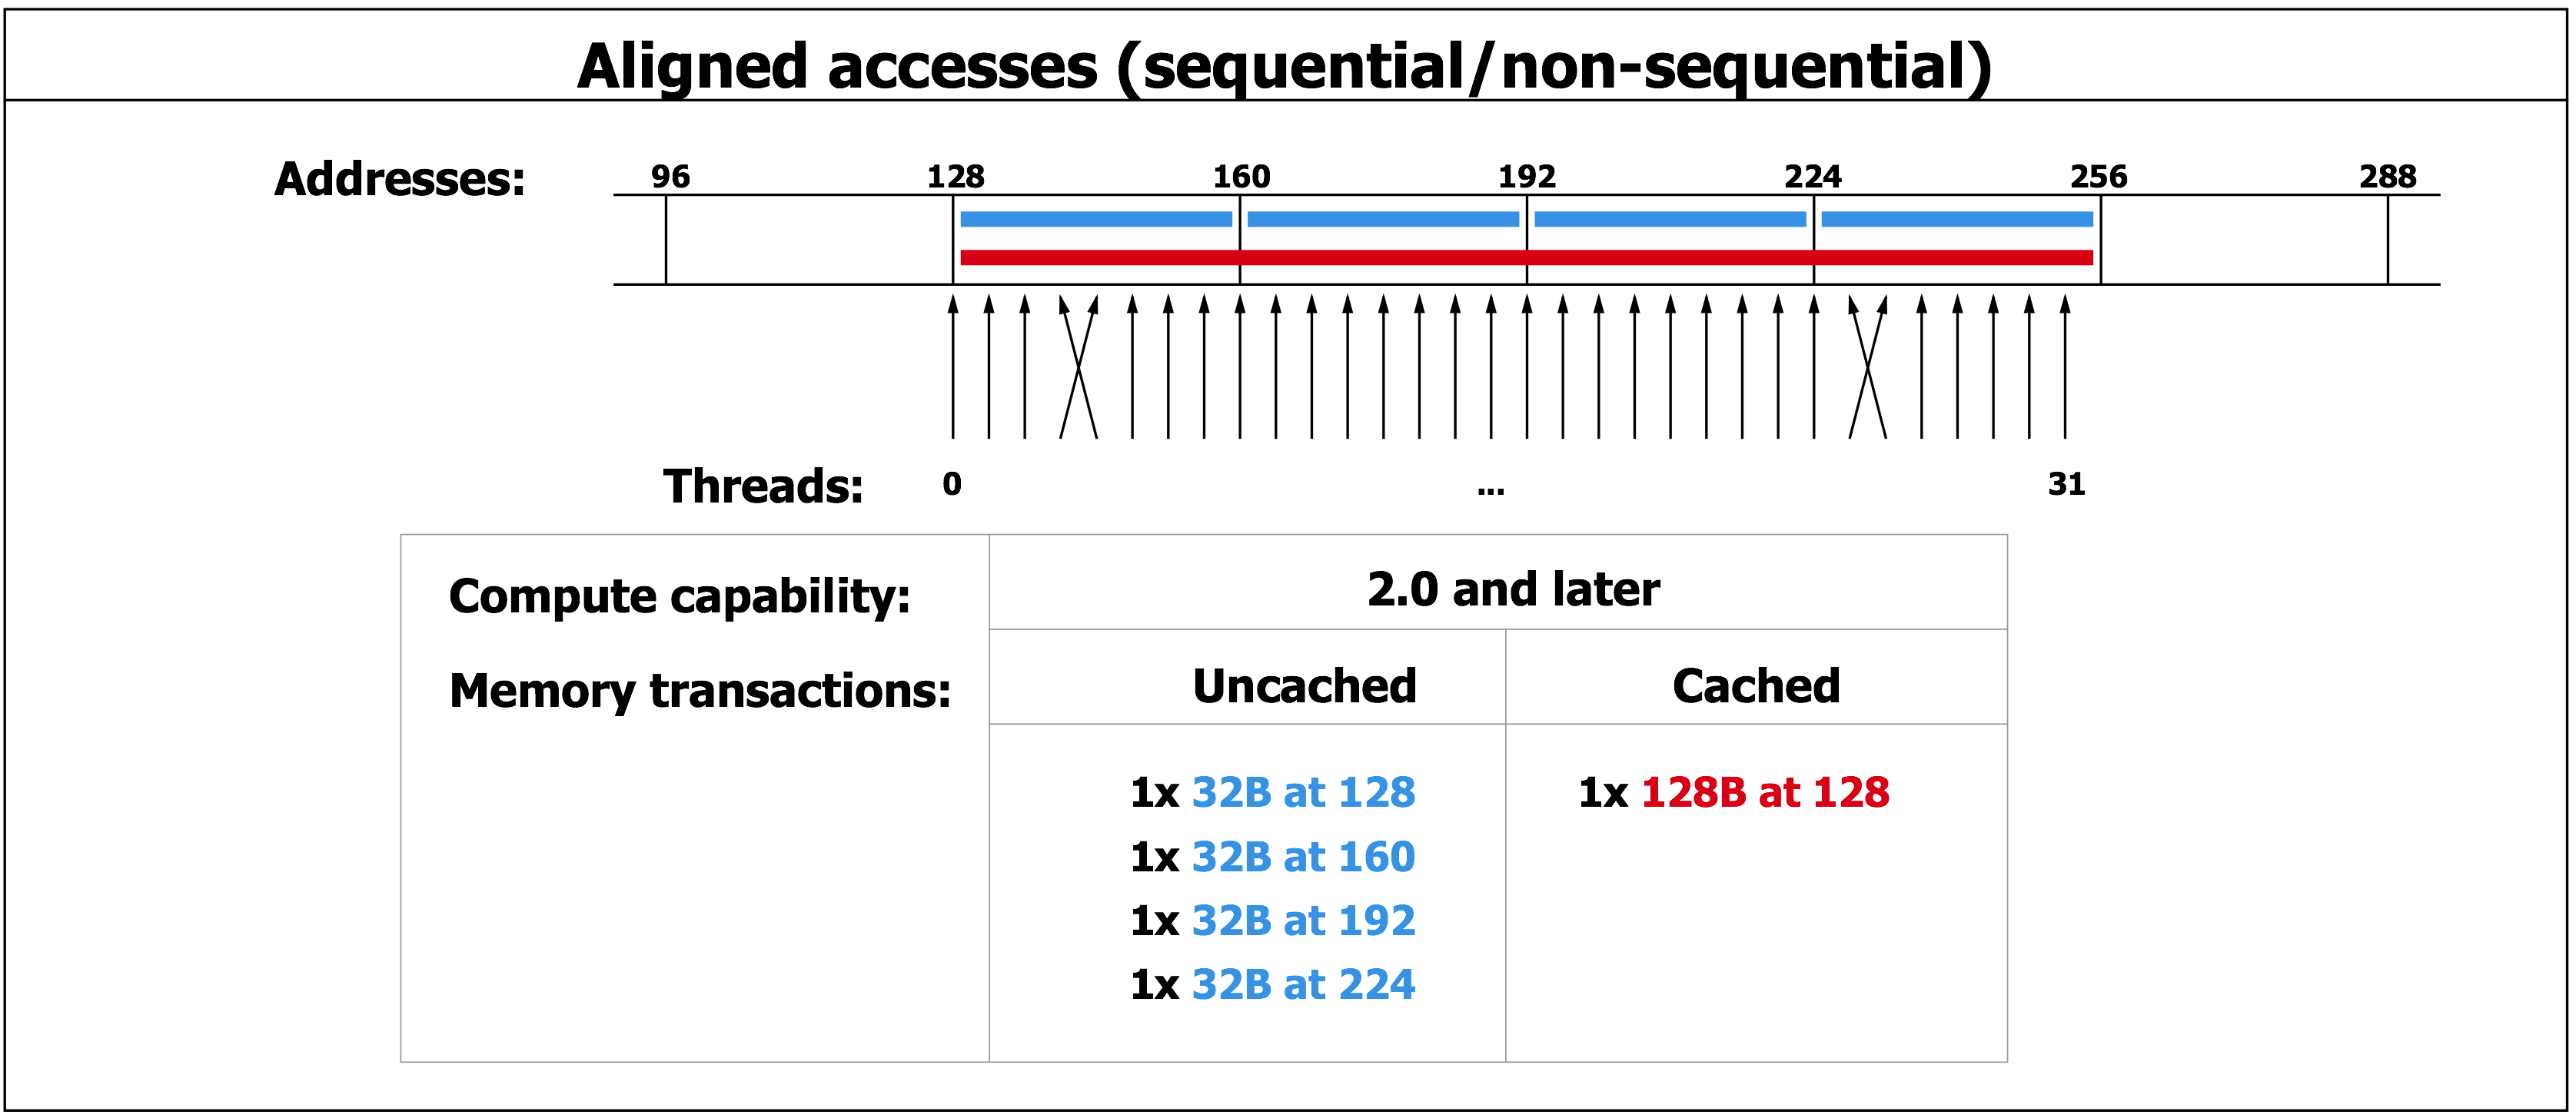
\includegraphics[height=0.7\textheight]{coa1}
	\end{figure}
\begin{itemize}
	\item[$\rightarrow$] 4 transactions per warp (uncached)
	\end{itemize}
\end{frame}

\begin{frame}[fragile]
	\frametitle{Misaligned Memory Accesses}
\begin{lstlisting}
int i = globalArray[threadIdx.x + 1];
\end{lstlisting}
		\begin{figure}
	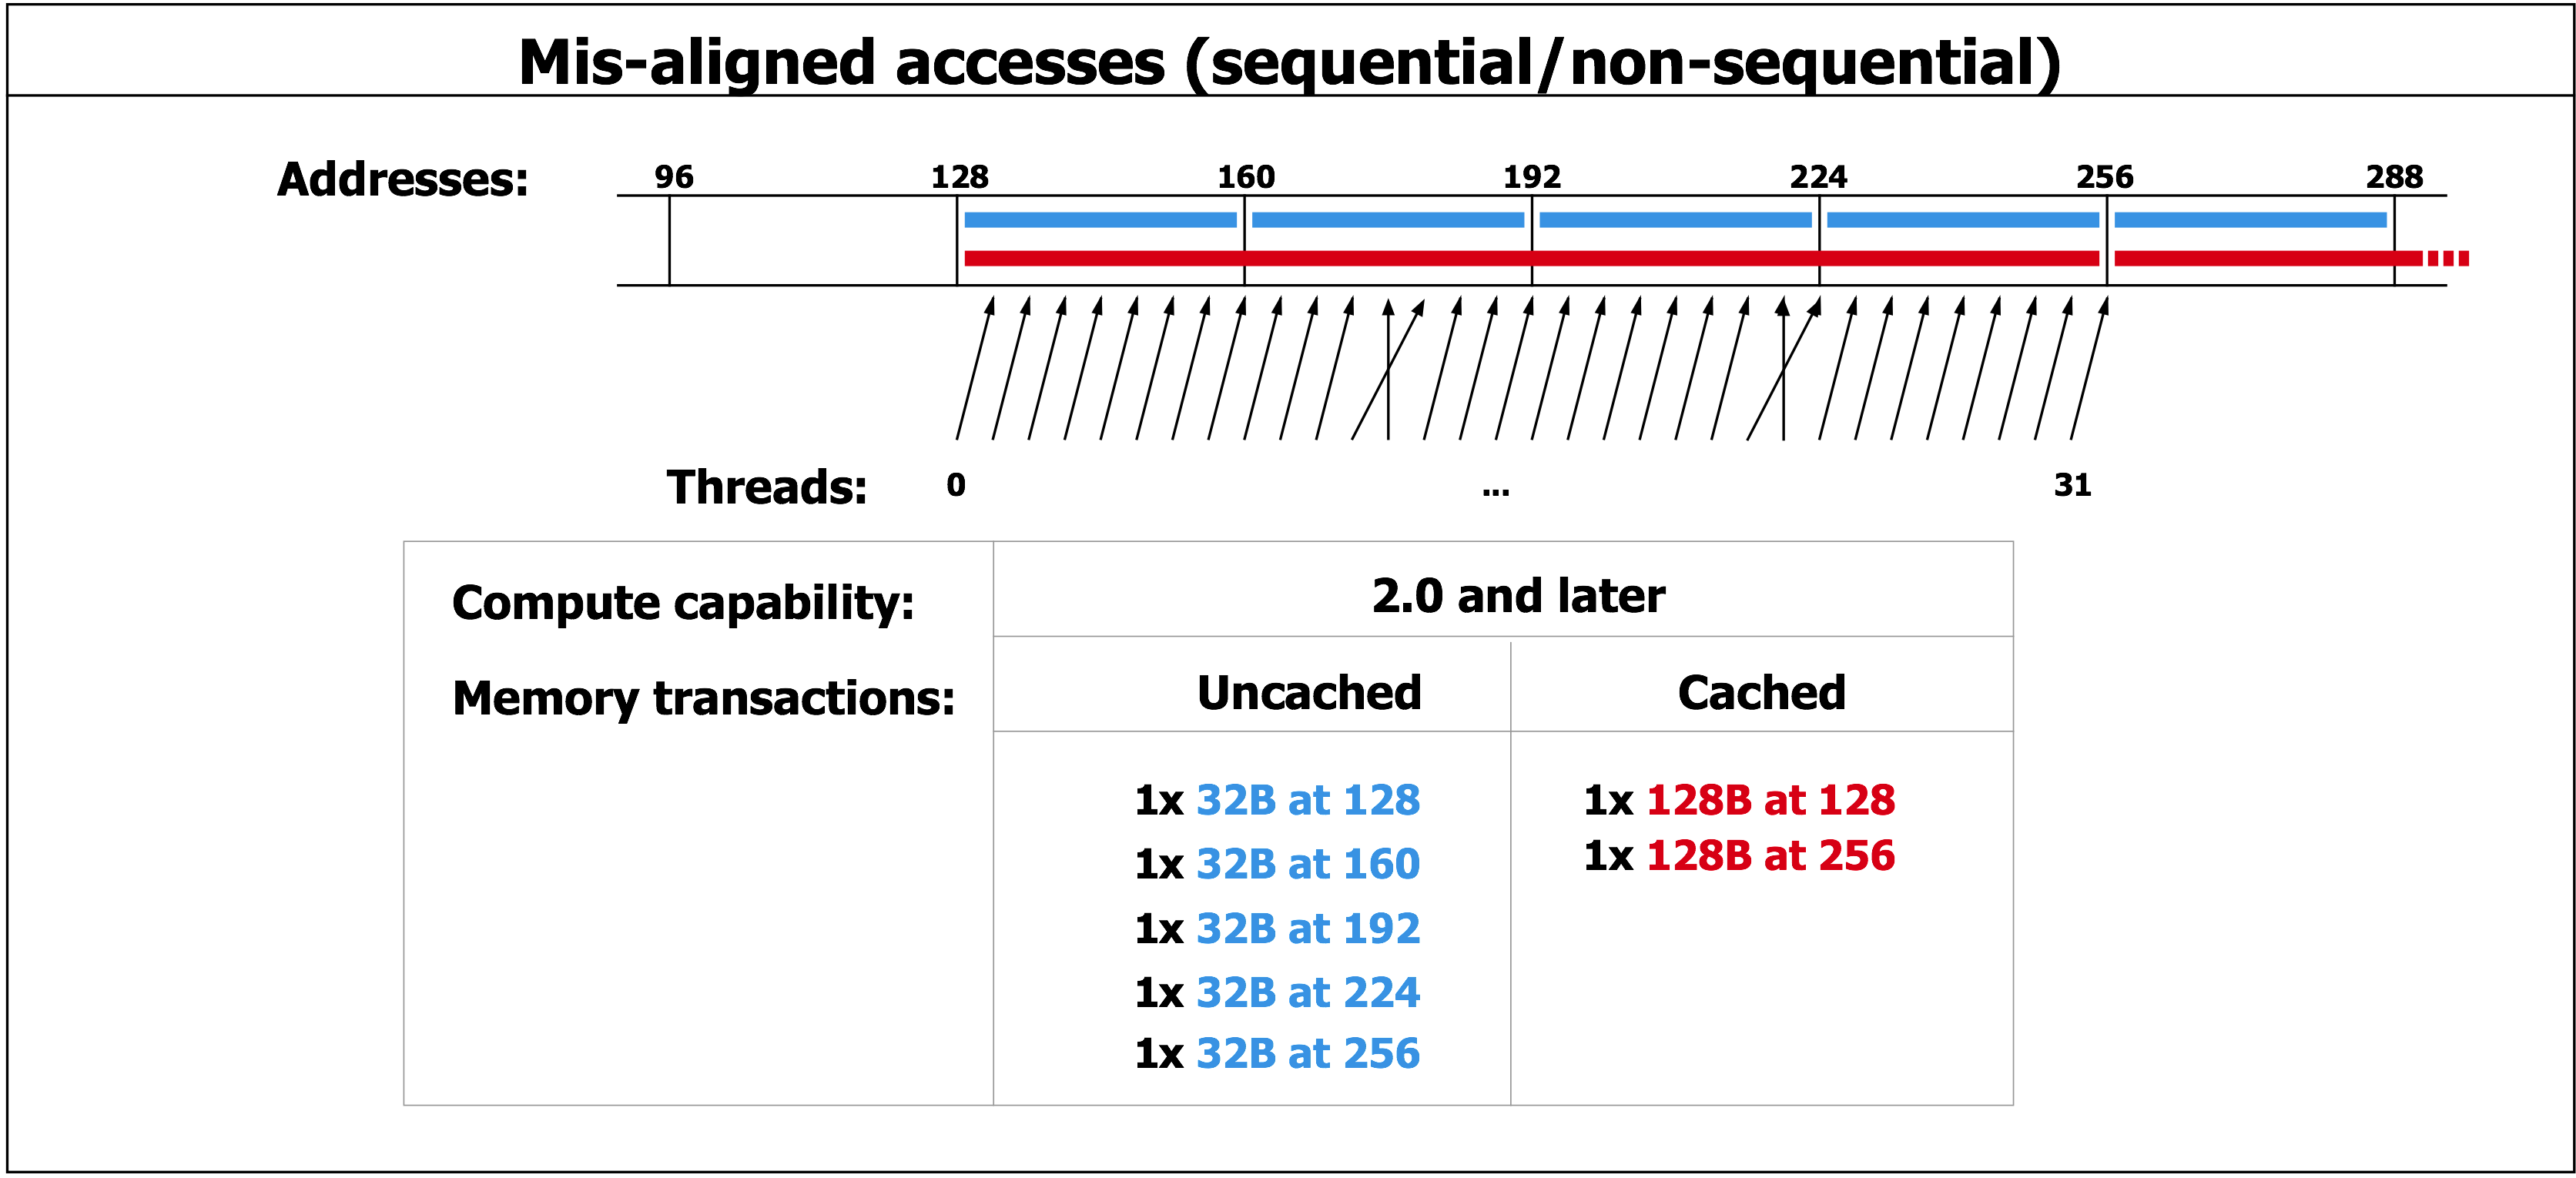
\includegraphics[height=0.7\textheight]{coa2}
\end{figure}
\begin{itemize}
	\item[$\rightarrow$] 5 transactions per warp (uncached), 25\% more than optimal
	\end{itemize}
\end{frame}


\begin{frame}[fragile]
	\frametitle{Strided Access 1}
	\begin{itemize}
	\item The read/written element is smaller than the gap between those elements
	\item Naturally occurs by accessing members of a struct
\end{itemize}
Example:
\begin{lstlisting}       
struct EIGEN_ALIGN32 Particle {
	vec4 position;
	vec4 velocity;
};  
// ...
vec4 p = particles[tid].position;
vec4 v = particles[tid].velocity;
// ...
\end{lstlisting} 
\end{frame}


\begin{frame}[fragile]
	\frametitle{Strided Access 2}
	\begin{itemize}
	\item 	\textbf{Non-coalescable memory access pattern}
\end{itemize}
	\begin{figure}
		\centering
		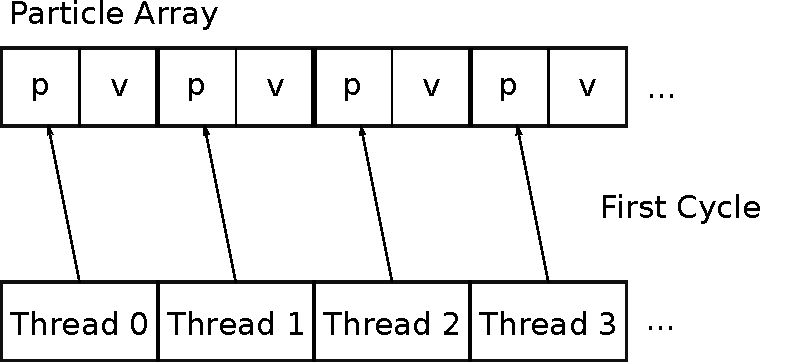
\includegraphics[height=0.5\textheight]{accessParticle1}
	\end{figure}
\begin{lstlisting}[language=bash]               
LD.E.128 R4, [R12];   
\end{lstlisting} 
\end{frame}


\begin{frame}[fragile]
	\frametitle{Strided Access 3}
	\begin{itemize}
		\item 	\textbf{Non-coalescable memory access pattern}
	\end{itemize}

	\begin{figure}
		\centering
		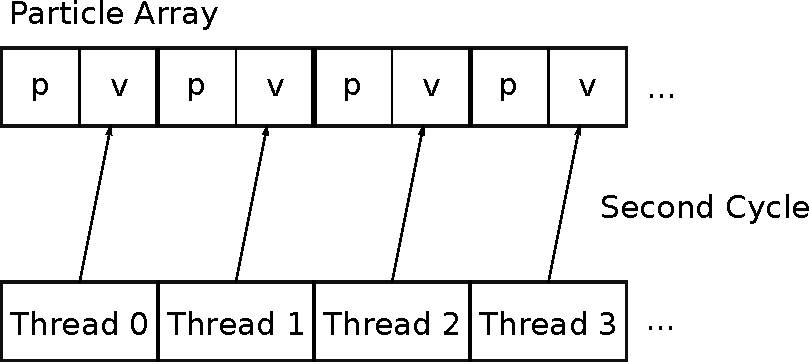
\includegraphics[height=0.5\textheight]{accessParticle2}
	\end{figure}
\begin{lstlisting}[language=bash]               
LD.E.128 R8, [R12+0x10];  
\end{lstlisting} 
\begin{itemize}
	\item[$\rightarrow$] 2 times more transactions than optimal
	\end{itemize}
\end{frame}

\begin{frame}[fragile]
\frametitle{Strided Access Solution}
Instead of storing and array of particles, we split it into
\begin{itemize}
	\item an array of positions
	\item an array of velocities
\end{itemize}
This concept is often called \textbf{structure of arrays} and is widely used in high performance computing and GPU libraries.
\begin{lstlisting}
vec4* positions = ...;
vec4* velocities = ...;
// ...
vec4 p = positions[tid];
vec4 v = velocities[tid];
// ...
\end{lstlisting}
\end{frame}



\begin{frame}[fragile]
\frametitle{Particle Integration Performance}
	\begin{tabular}{l|l|l|l}
	\textbf{Method} & \textbf{Time (ms)} & \textbf{Bandwidth (GB/s)} & \textbf{Speed Up} \\	
	\hline
	Initial & 0.458  & 139.509 & 1 \\
	Vector + Inverse Layout & 0.273  &       233.918 & 1.68 \\
	Vector + Shared LS & 0.274   &    233.209 & 1.68 \\
	cudaMemcpy & 0.275   &    232.342 & 1.68  
\end{tabular}
\\
\vspace{0.5cm}
\begin{itemize}
	\item[$\rightarrow$] Optimizing the global memory access improves performance by around 68\%
	\item[$\rightarrow$] We have reached bandwidth limit (same BW as cudaMemcpy)
	\item[$\rightarrow$] \href{https://github.com/darglein/saiga/blob/master/samples/cuda/globalMemory/main.cu}{Full source code @ GitHub}
\end{itemize}
\end{frame}


\begin{frame}[fragile]
\frametitle{Profiling}
First, make sure the profiling timeline is consistent
\begin{itemize}
	\item The simulation is initialized correctly
	\item The simulation runs for a fixed amount of steps
	\item No user input is required during a simulation
\end{itemize}
Enable the \texttt{CUDA\_PROFILING} flag in CMake
\begin{lstlisting}[language=bash]
cmake -DCUDA_PROFILING=ON ..
\end{lstlisting}
\end{frame}


\begin{frame}[fragile]
\frametitle{Profiling}
Profile only a single simulation step:

\begin{lstlisting}
#ifdef CUDA_PROFILING
static int steps = 0;
if(steps == 300) cudaProfilerStart();
#endif

// The actual simulation step
particleSystem->update();

#ifdef CUDA_PROFILING
if(steps++ == 300){
	cudaProfilerStop();
	parentWindow.close();
}
#endif

\end{lstlisting}
\end{frame}




\begin{frame}[fragile]
\frametitle{Profiling}

	\begin{minipage}{0.5\linewidth}
		\begin{enumerate}
			\item 		Launch the NVidia Visual Profiler (NVVP)
\begin{lstlisting}[language=bash]
nvvp ./agphys
\end{lstlisting}
			\item Uncheck \textit{Start execution with profiling enabled}
			\item[$\rightarrow$] We only profile one step
			\item Uncheck \textit{Unified memory profiling}
			\item[$\rightarrow$] Requires \textit{root}
			\item Click finish
		\end{enumerate}


\end{minipage}
\begin{minipage}{0.47\linewidth}

\end{minipage}
\end{frame}


\begin{frame}[fragile]
\frametitle{Occupancy}

%https://docs.nvidia.com/gameworks/content/developertools/desktop/analysis/report/cudaexperiments/kernellevel/achievedoccupancy.htm
	\begin{mdframed}[frametitle={CUDA Programming Guide}]
A warp is considered active from the time its threads begin executing to the time when all threads in the warp have exited from the kernel. There is a maximum number of warps which can be concurrently active on a Streaming Multiprocessor (SM). \textbf{Occupancy is defined as the ratio of active warps on an SM to the maximum number of active warps supported by the SM.}
\end{mdframed}
\end{frame}


\begin{frame}[fragile]
\frametitle{Occupancy Limiting Factors}
\textbf{Warps per SM}
\begin{itemize}
	\item The SM has a maximum number of warps that can be active at once. 
	\item For most current GPUs this limit is 64 (=2048 Threads)
\end{itemize}

\textbf{Blocks per SM}
\begin{itemize}
	\item The SM has a maximum number of blocks that can be active at once.
	\item A typical limit is 32 blocks per SM $\rightarrow$ Minimum block size is 64 threads
\end{itemize}		
\end{frame}

\begin{frame}[fragile]
\frametitle{Occupancy Limiting Factors}
\textbf{Registers per SM}
\begin{itemize}
	\item The SM has a set of registers shared by all active threads.
	\item For most current GPUs this limit is 65536 (32 registers per active thread)
\end{itemize}

\textbf{Shared Memory per SM}
\begin{itemize}
	\item The SM has a fixed amount of shared memory shared by all active threads. 
	\item The L1 cache resides in shared memory
	\item For current GPUs the limit is 98304 bytes (12 $\times$ 4 byte per active thread)
\end{itemize}		
\end{frame}


\begin{frame}[fragile]
\frametitle{Occupancy}
When does occupancy \textbf{not} matter?
\begin{itemize}
	\item For bandwidth limited kernels
	\item For compute bound kernels
\end{itemize}

When does occupancy matter?
\begin{itemize}
	\item For latency bound kernels
\end{itemize}		
\end{frame}



\begin{frame}[fragile]
\frametitle{Latency}

Similar to CPU threads, active warps can be either \textbf{running}, \textbf{ready} or \textbf{blocked}.
\begin{itemize}
	\item A running warp executes commands until a blocking instruction
	\item A blocked warp waits for an event
	\item A ready warp waits until a running warp stops 
	\item A running warp is never stopped by the scheduler
\end{itemize}

	\begin{figure}
	\centering
	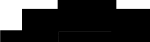
\includegraphics[height=0.3\textheight]{latency}
\end{figure}
\end{frame}


\begin{frame}[fragile]
\frametitle{Latency}

\begin{itemize}
	\item SMs on current GPUs can have 4 warps running at the same time
	\item Each SM can have 64 active warps
	\item[$\rightarrow$] With high occupancy, memory latency can be hidden by the scheduler
	\item[$\rightarrow$] With low occupancy, less than 3 warps might be running at the same time
\end{itemize}
\end{frame}



\begin{frame}[fragile]
\frametitle{Occupancy Example}

\begin{minipage}{0.5\linewidth}
	Particle-Particle Collision Kernel
	\begin{itemize}
		\item Uses 40 registers/thread
		\item Occupancy: 75\%
		\item Latency issues because of acceleration structure
		\item[$\rightarrow$] Higher occupancy could increase performance
		\item[$\rightarrow$] Try to reduce registers to 32/thread
	\end{itemize}
\end{minipage}
\begin{minipage}{0.47\linewidth}

\end{minipage}
\end{frame}


\begin{frame}[fragile]
\frametitle{Launch Bounds}
	The register usage can be controlled by the \texttt{\_\_launch\_bounds\_\_} intrinsic. \\
	\textbf{Syntax:}
\begin{lstlisting}
__launch_bounds__(MAX_THREADS_PER_BLOCK,MIN_BLOCKS_PER_SM)
\end{lstlisting}
\textbf{Example:}
\begin{lstlisting}
template<unsigned int BLOCK_SIZE>
__launch_bounds__(BLOCK_SIZE,MAX_THREADS_PER_SM/BLOCK_SIZE)
__global__ static
void collideParticlesLCK(...)
{
 	//...
}
\end{lstlisting}

\end{frame}


\begin{frame}[fragile]
\frametitle{Occupancy Example}

\begin{minipage}{0.5\linewidth}
	With launch bounds we achieve
	\begin{itemize}
		\item Uses 32 registers/thread
		\item Occupancy: 100\%
		\item 5\% \textbf{worse} performance
		\item[$\rightarrow$] The kernel uses local memory now
	\end{itemize}
\end{minipage}
\begin{minipage}{0.47\linewidth}

\end{minipage}
\end{frame}


\begin{frame}[fragile]
\frametitle{Advanced Profiling}

	\begin{enumerate}
		\item Switch to unguided analysis
		\item Run Global Memory analysis
		\item Click on individual transaction
	\end{enumerate}
	
\end{frame}




\frame{
	\frametitle{Literature}
	%
	\begin{itemize}
		\item \href{https://docs.nvidia.com/cuda/}{Cuda Toolkit Documentation}
		\item \href{https://docs.nvidia.com/cuda/cuda-driver-api/}{CUDA driver API}
		\item \href{https://docs.nvidia.com/cuda/cuda-runtime-api/}{ CUDA runtime API}
	\end{itemize}
	
}





\end{document}



